\documentclass[palatino]{beamer}

\usepackage{psfrag}
\usepackage{graphics}
\usepackage{latexsym}
\usepackage{amsfonts}
\usepackage{amsmath}	
\usepackage{bm}
\usepackage{epstopdf}
\usepackage{tikz}

\usepackage{hyperref} 
\hypersetup{colorlinks=true, linkcolor=white,  anchorcolor=blue,  
citecolor=blue, filecolor=blue, menucolor=blue, pagecolor=blue,  
urlcolor=blue,pdftitle={ACmain}}

\definecolor{royalblue}{rgb}{.2,.6,1}%
\definecolor{mygrey}{rgb}{.64,.64,.64}%
\definecolor{mywhite}{rgb}{1,1,1}%
\definecolor{mypurple}{rgb}{.8,.6,1}%

\definecolor{red}{rgb}{1,0,0}
\definecolor{skyblue}{rgb}{0.1960, 0.6000, 0.8000}

\mode<presentation>
{
% THEME CHOICES
%\usetheme{Warsaw}
%\usetheme{Rochester}
%\usetheme{Bergen}
%\usetheme{Berlin}
\usetheme{Copenhagen}
%\usetheme{Madrid}
%\usetheme{PaloAlto}

% SET BACKGROUND COLORS

\setbeamercolor{background canvas}{bg=mywhite}
\setbeamerfont{frametitle}{size=\large}
}

\setbeamercolor{frame}{bg=mygold}

\usepackage[english]{babel}

\usepackage[latin1]{inputenc}

\usepackage{palatino}

\title[Exam 1 Review] 
{Conceptual Questions: Exam 1 Review}

\author[MTH 210 -- Talbert]{MTH 210: Communicating in Mathematics \\ Prof. Talbert} 

  \date{Sept 28, 2012}

\AtBeginSubsection[]


\begin{document}
	
	\begin{frame}
	  \titlepage
	\end{frame}

	
%  FOR THE FIRST TIME WE DO CLICKER QUESTIONS: 
% 	
% \begin{frame}{Notes on clicker questions}
% 	\begin{itemize}
% 		\item You'll be presented with a question and asked to read it. Polling will then be opened. 
% 		\item Click the letter corresponding to the answer you feel is most correct. If you change your mind before time is up, click again and your first vote will be over-written. 
% 		\item You get 1 minute to decide and vote. If your clicker gives a green light, your vote has been received. 
% 		\item \textbf{You are not being graded on whether you have a right answer or not. }
% 		\item But, you must click every time we vote in order to get participation credit. 
% 		\item After one vote, if there is not a consensus, we'll break into small groups for discussion and then vote again. 
% 	\end{itemize}
% \end{frame}	
% 	

\begin{frame}
Which of the following are you allowed to use during Exam 1?
\begin{enumerate}[(a)]
	\item A pen
	\item A $3 \times 5$ notecard with notes on it
	\item An iPod touch calculator app
	\item All of the above
	\item Jut (a) and (b)
	\item None of the above
\end{enumerate}
\end{frame}

\begin{frame}
Which of the following are statements? 
\begin{enumerate}[(a)]
	\item $3^2 + 4^2 = 5^2$. 
	\item $a^2 + b^2 = c^2$. 
	\item If $x^2 = 4$, then $x = 2$. 
	\item Every square is a rectangle. 
	\item All of the above
	\item Three of the above (specify)
	\item Two of the above (specify)
\end{enumerate}
\end{frame}


\begin{frame}
	Consider the statement
	\begin{quote}
		If $8 < 5$, then $a + 2 = 10$. 
	\end{quote}
This statement is true
\begin{enumerate}[(a)]
	\item Always
	\item Sometimes (depends on $a$)
	\item Never
\end{enumerate}
\end{frame}

\begin{frame}
	Every conditional statement $P \rightarrow Q$ is logically equivalent to
	\begin{enumerate}[(a)]
		\item Its converse
		\item Its contrapositive
		\item Its negation
		\item Its equivalent biconditional statement $P \leftrightarrow Q$
		\item More than one of the above (be ready to specify)
	\end{enumerate}
\end{frame}

\begin{frame}
	The negation of $P \rightarrow Q$ is 
	\begin{enumerate}[(a)]
		\item $\neg P \rightarrow Q$
		\item $P \rightarrow \neg Q$
		\item $P \vee \neg Q$
		\item $\neg P \wedge Q$
		\item None of the above
	\end{enumerate}
\end{frame}


\begin{frame}
	Let $A = \{ 2, 4, 6, 8\}$ and $B = \{ x \in \mathbb{N} \, | \, x^2 < 100 \}$. Then
	\begin{enumerate}[(a)]
		\item $A \subseteq B$
		\item $B \subseteq A$
		\item $A = B$
		\item All of the above
		\item None of the above
	\end{enumerate}
\end{frame}


\begin{frame}
	Consider the predicate ``$n$ is prime and congruent to $0 \pmod 4$''. The truth set of this statement is 
	\begin{enumerate}[(a)]
		\item $\mathbb{Z}$
		\item The set of all prime numbers
		\item The set of all natural numbers divisible by $4$
		\item $\{ 2 \}$
		\item $\emptyset$ (the empty set)
	\end{enumerate}

\end{frame}

\begin{frame}
	Consider the statement: 
	\begin{quote}
		There exists no prime number that is congruent to $0$ modulo $4$. 
	\end{quote}
The negation of this statement would say
\begin{enumerate}[(a)]
	\item There exists a prime number that is congruent to $0$ modulo $4$.
	\item There exists a prime number that is not congruent  to $0$ modulo $4$.
	\item Every prime number is congruent to $0$ modulo $4$.
	\item Every prime number fails to be congruent to $0$ modulo $4$. 
\end{enumerate}
\end{frame}


\begin{frame}
What is the smallest nonnegative integer that is congruent to 1179 modulo 10?
\begin{enumerate}[(a)]
	\item $0$
	\item $1$
	\item $9$
	\item $79$
	\item This number does not exist
\end{enumerate}
\end{frame}

\begin{frame}
	Suppose $a \equiv 0 \pmod {12}$. Then
	\begin{enumerate}[(a)]
		\item $a$ divides $12$
		\item $a$ is even
		\item $a$ is divisible by $6$
		\item All of the above
		\item Just (b) and (c)
	\end{enumerate}
\end{frame}

\begin{frame}
	Consider the statement:
	\begin{quote}
		If $a \equiv 0 \pmod {12}$, then $6 | a$. 
	\end{quote}
If you tried to prove this using proof by contraposition, you would assume
	\begin{enumerate}[(a)]
		\item $a \equiv 0 \pmod {12}$
		\item $a \not \equiv 0 \pmod {12}$
		\item $6 | a$
		\item $6 \not | a$
		\item $a \equiv 0 \pmod {12}$ and $6 \not | a$
	\end{enumerate}
\end{frame}

\begin{frame}
	Consider the statement:
	\begin{quote}
		If $a \equiv 5 \pmod {12}$, then $a^2 \equiv 1 \pmod {12}$. 
	\end{quote}
If you wanted to use cases in a direct proof of this statement, which of the following sets of cases are valid? 
	\begin{enumerate}[(a)]
		\item Two cases: $a \geq 0$ and $a < 0$
		\item Two cases: $a$ prime and $a$ not prime
		\item Three cases: $a < 0$, $0 \leq a < 11$, and $a \geq 12$
		\item All of the above
	\end{enumerate}
\end{frame}

\begin{frame}{Proof Analysis}
	
For each of the following proofs, read carefully and then vote: 
\begin{enumerate}
	\item The proposition is false (and therefore the ``proof'' cannot be correct)
	\item The proposition is true, but the proof is wrong 
	\item The proposition is true and the proof is right, but the proof needs improvement
	\item The proposition is true and the proof needs no correction
\end{enumerate}
	
\end{frame}

\begin{frame}
	\begin{center}
		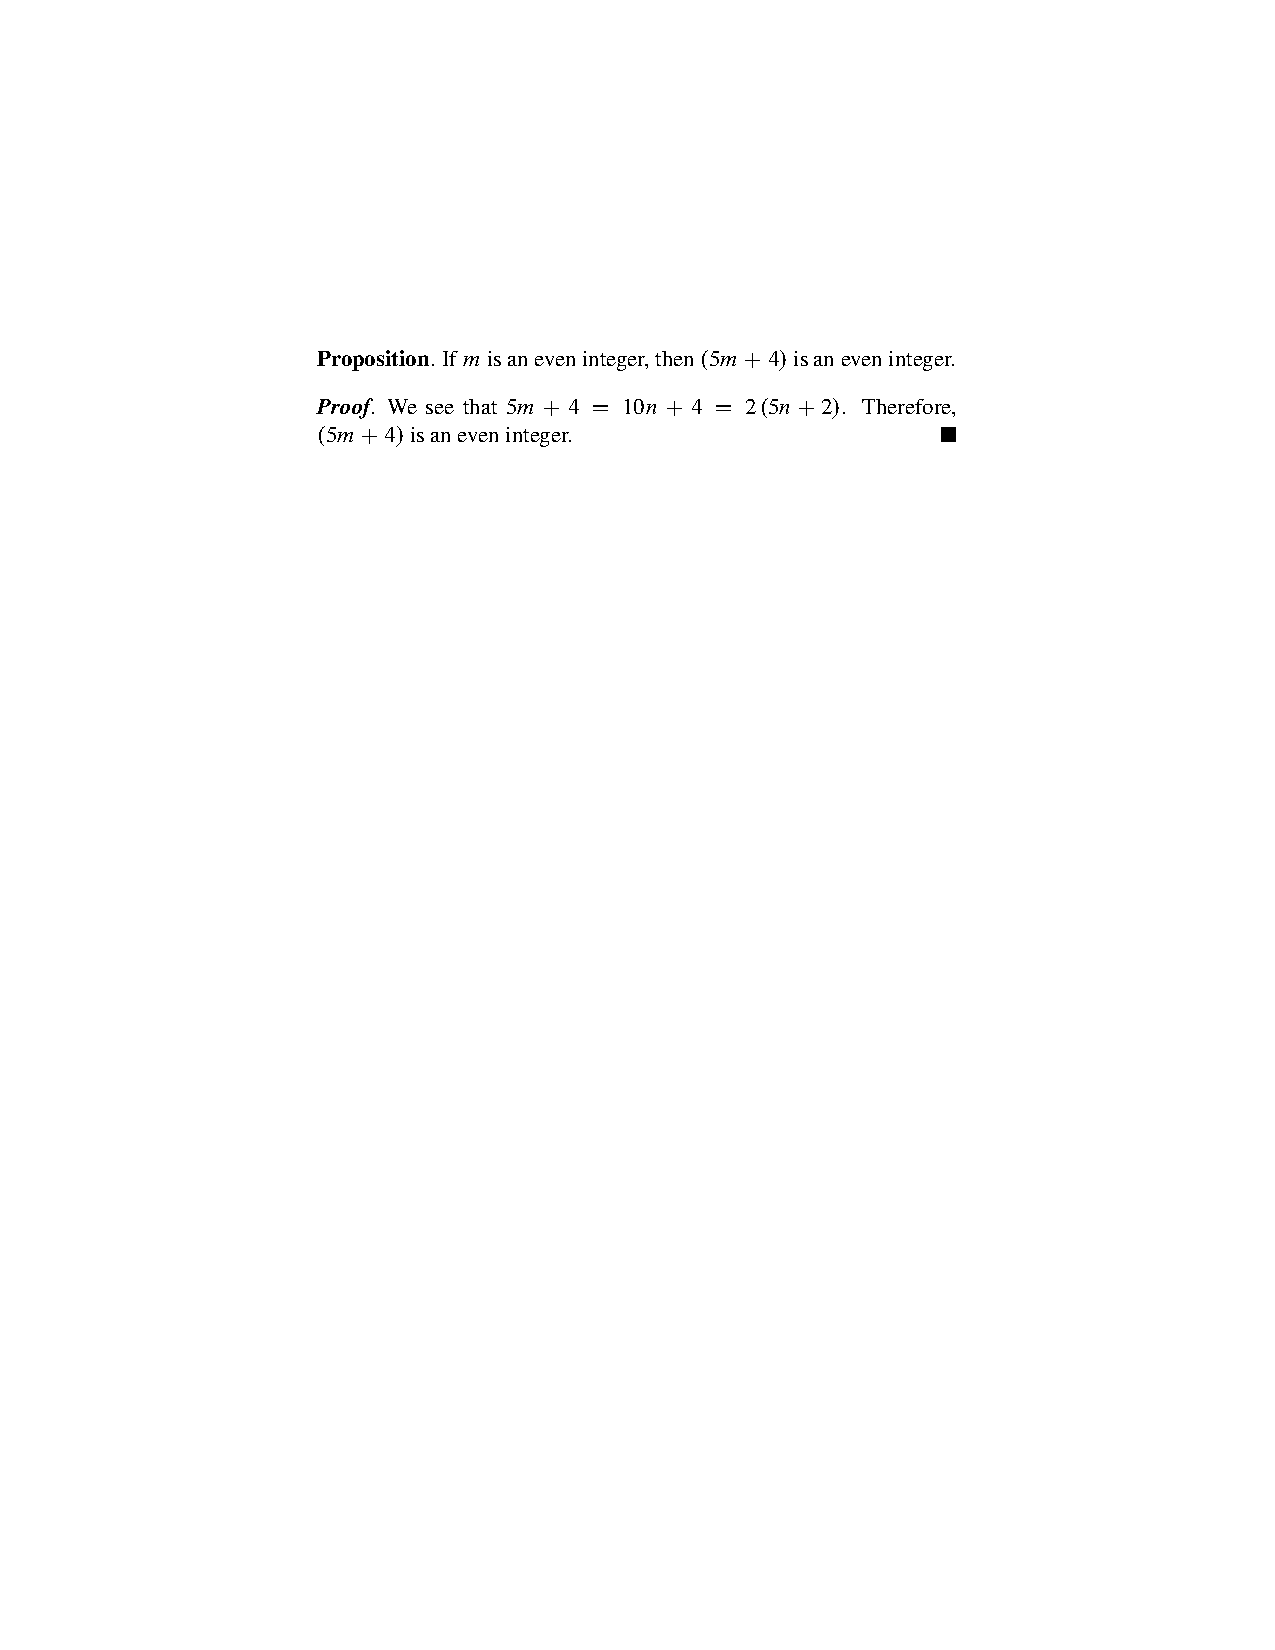
\includegraphics[width=4in]{exam1-proofanalysis4}
	\end{center}
\end{frame}


\begin{frame}
	\begin{center}
		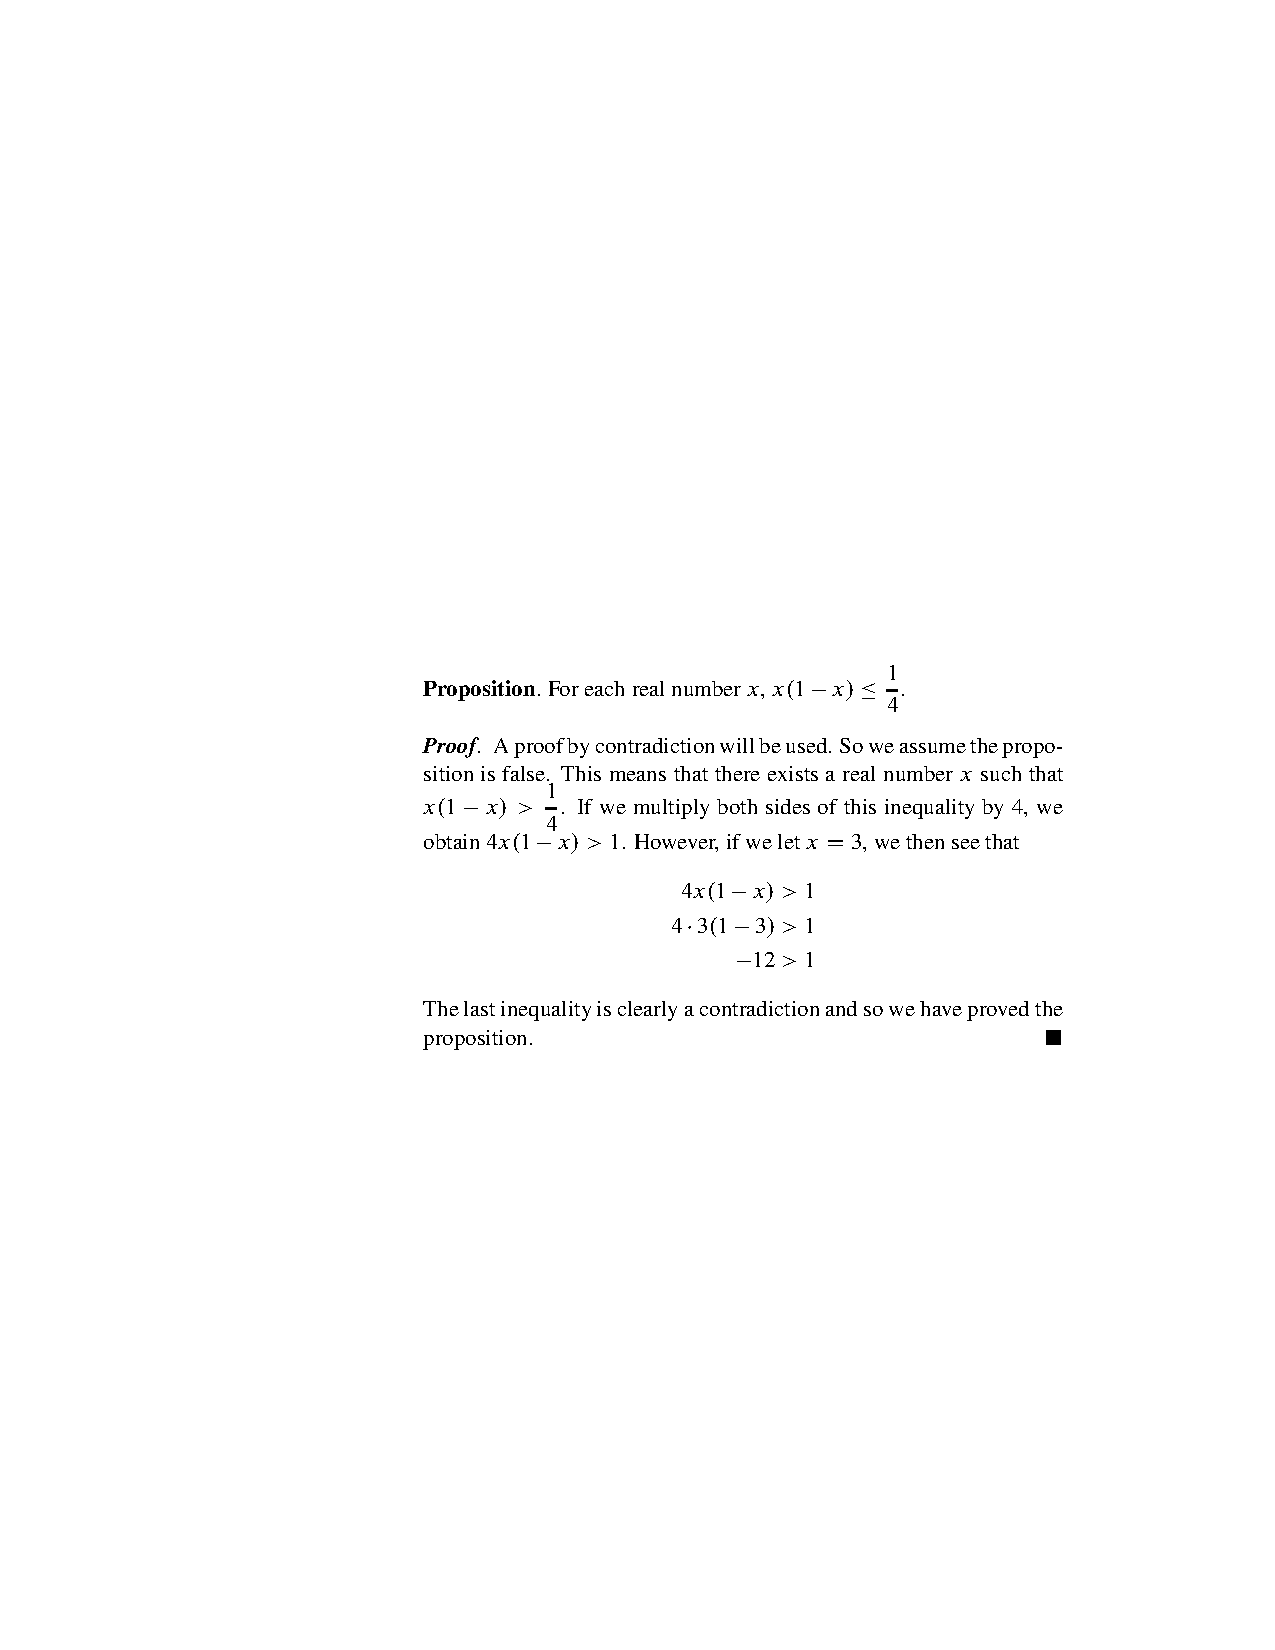
\includegraphics[width=4in]{exam1-proofanalysis2}
	\end{center}
\end{frame}

\begin{frame}
	\begin{center}
		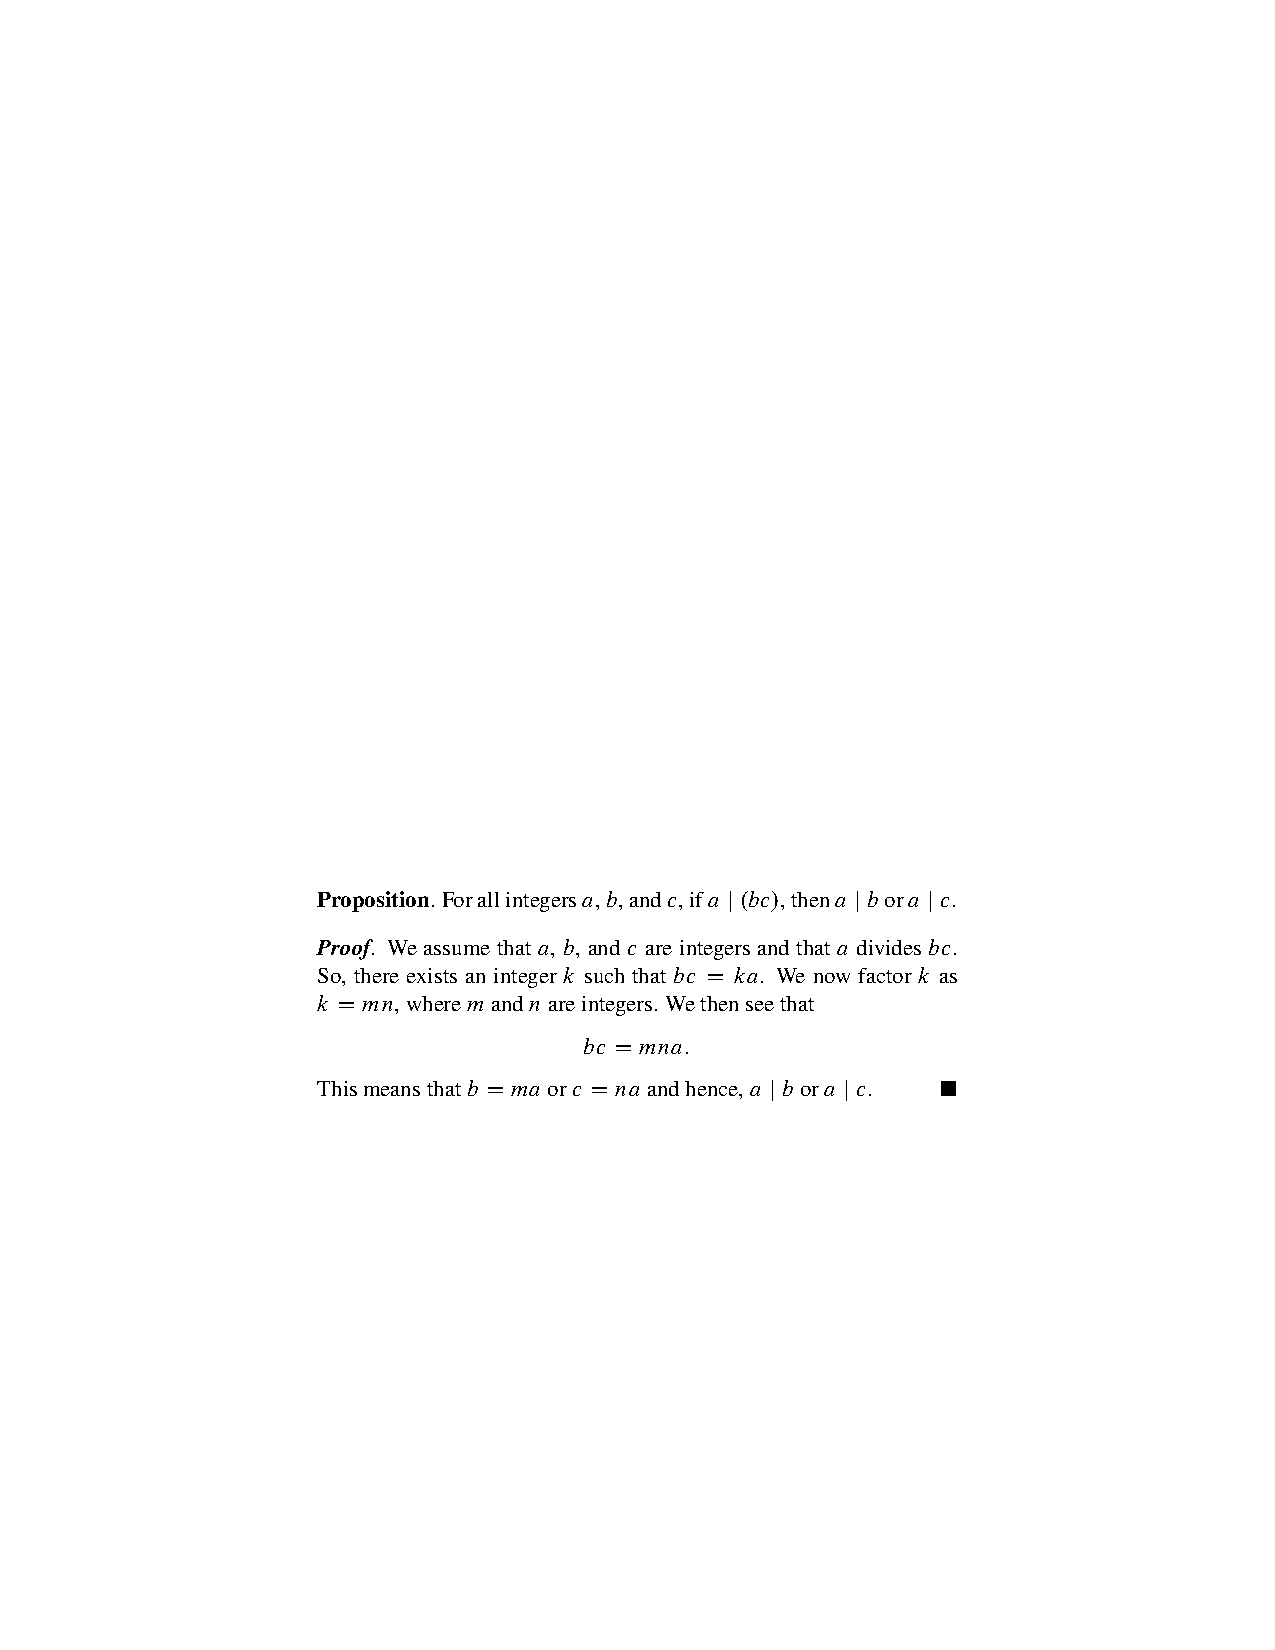
\includegraphics[width=4in]{exam1-proofanalysis3}
	\end{center}
\end{frame}


\end{document}